\documentclass[
	ngerman,
	aspectratio=169,
	color={accentcolor=3d},
	logo=false,
	colorframetitle=true,
%	logofile=example-image,
	]{tudabeamer}

\usepackage{amsmath}
\usepackage{amsfonts}
\usepackage{amssymb}
\usepackage[main=english]{babel}
\usepackage{graphicx}
\usepackage{physics}
\usepackage{subcaption}
\usepackage{tikz}
\usetikzlibrary{arrows.meta, shadings, shadows, shapes, arrows}
\usepackage[numbers]{natbib}
\usepackage{pifont}
\usepackage{comment}

\hypersetup{pagebackref=true,breaklinks=true,colorlinks,bookmarks=false,citecolor=magenta,linkcolor=magenta}

\newcommand{\cmark}{\ding{51}}
\newcommand{\xmark}{\ding{55}}

\definecolor{tud0d}{cmyk/RGB/HTML}{0,0,0,.8/83,83,83/535353}
\definecolor{tud0c}{cmyk/RGB/HTML}{0,0,0,.6/137,137,137/898989}
\definecolor{tud0b}{cmyk/RGB/HTML}{0,0,0,.4/181,181,181/B5B5B5}
\definecolor{tud0a}{cmyk/RGB/HTML}{0,0,0,.2/220,220,220/DCDCDC}
\definecolor{tud1a}{cmyk/RGB/HTML}{.7,.4,0,0/93,133,195/5D85C3}
\definecolor{tud2a}{cmyk/RGB/HTML}{0.8,.2,0,0/0,156,218/009CDA}
\definecolor{tud3a}{cmyk/RGB/HTML}{0.7,0,.5,0/80,182,149/50B695}
\definecolor{tud4a}{cmyk/RGB/HTML}{.4,0,.8,0/175,204,80/AFCC50}
\definecolor{tud5a}{cmyk/RGB/HTML}{.2,0,.8,0/221,223,72/DDDF48}
\definecolor{tud6a}{cmyk/RGB/HTML}{0,.1,.7,0/255,224,92/FFE05C}
\definecolor{tud7a}{cmyk/RGB/HTML}{0,.3,.8,0/248,186,60/F8BA3C}
\definecolor{tud8a}{cmyk/RGB/HTML}{0,.6,.8,0 /238,122,52/EE7A34}
\definecolor{tud9a}{cmyk/RGB/HTML}{0,.8,.7,0/233,80,62/E9503E}
\definecolor{tud10a}{cmyk/RGB/HTML}{.2,.9,0,0/201,48,142/C9308E}
\definecolor{tud11a}{cmyk/RGB/HTML}{.6,.8,0,0/128,69,151/804597}
\definecolor{tud1b}{cmyk/RGB/HTML}{1,.6,0,0/0,90,169/005AA9}
\definecolor{tud2b}{cmyk/RGB/HTML}{1,.3,0,0/0,131,204/0083CC}
\definecolor{tud3b}{cmyk/RGB/HTML}{1,0,.6,0/0,157,129/009D81}
\definecolor{tud4b}{cmyk/RGB/HTML}{.5,0,1,0/153,192,0/99C000}
\definecolor{tud5b}{cmyk/RGB/HTML}{.3,0,1,0/201,212,0/C9D400}
\definecolor{tud6b}{cmyk/RGB/HTML}{0,.2,1,0/253,202,0/FDCA00}
\definecolor{tud7b}{cmyk/RGB/HTML}{0,.4,1,0/245,163,0/F5A300}
\definecolor{tud8b}{cmyk/RGB/HTML}{0,.7,1,0/236,101,0/EC6500}
\definecolor{tud9b}{cmyk/RGB/HTML}{0,1,.9,0/230,0,26/E6001A}
\definecolor{tud10b}{cmyk/RGB/HTML}{.4,1,0,0/166,0,132/A60084}
\definecolor{tud11b}{cmyk/RGB/HTML}{.7,1,0,0/114,16,133/721085}
\definecolor{tud1c}{cmyk/RGB/HTML}{1,.7,.2,0/0,78,138/004E8A}
\definecolor{tud2c}{cmyk/RGB/HTML}{1,.5,.2,0/0,104,157/00689D}
\definecolor{tud3c}{cmyk/RGB/HTML}{1,.2,.6,0/0,136,119/008877}
\definecolor{tud4c}{cmyk/RGB/HTML}{.6,.1,1,0/127,171,22/7FAB16}
\definecolor{tud5c}{cmyk/RGB/HTML}{.4,.1,1,0/177,189,0/B1BD00}
\definecolor{tud6c}{cmyk/RGB/HTML}{.2,.3,1,0/215,172,0/D7AC00}
\definecolor{tud7c}{cmyk/RGB/HTML}{.2,.5,1,0/210,135,0/D28700}
\definecolor{tud8c}{cmyk/RGB/HTML}{.2,.8,1,0/204,76,3/CC4C03}
\definecolor{tud9c}{cmyk/RGB/HTML}{.3,1,.9,0/185,15,34/B90F22}
\definecolor{tud10c}{cmyk/RGB/HTML}{.5,1,.3,0/149,17,105/951169}
\definecolor{tud11c}{cmyk/RGB/HTML}{.8,1,.2,0/97,28,115/611C73}
\definecolor{tud1d}{cmyk/RGB/HTML}{1,.9,.3,0/36,53,114/243572}
\definecolor{tud2d}{cmyk/RGB/HTML}{1,.7,.4,0/0,78,115/004E73}
\definecolor{tud3d}{cmyk/RGB/HTML}{1,.4,.7,0/0,113,94/00715E}
\definecolor{tud4d}{cmyk/RGB/HTML}{.7,.3,1,0/106,139,55/6A8B22}
\definecolor{tud5d}{cmyk/RGB/HTML}{.5,.2,1,0/153,166,4/99A604}
\definecolor{tud6d}{cmyk/RGB/HTML}{.4,.4,1,0/174,142,0/AE8E00}
\definecolor{tud7d}{cmyk/RGB/HTML}{.3,.6,1,0/190,111,0/BE6F00}
\definecolor{tud8d}{cmyk/RGB/HTML}{.4,.8,1,0/169,73,19/A94913}
\definecolor{tud9d}{cmyk/RGB/HTML}{.5,1,.9,0/156,28,38/961C26}
\definecolor{tud10d}{cmyk/RGB/HTML}{.7,1,.5,0/115,32,84/732054}
\definecolor{tud11d}{cmyk/RGB/HTML}{.9,1,.3,0/76,34,106/4C226A}

% \setbeamercovered{dynamic}
\setbeamercovered{invisible}

\newcommand{\Vector}[1]{\boldsymbol{#1}}
\newcommand{\Matrix}[1]{\boldsymbol{\MakeUppercase{#1}}}
\newcommand{\Tensor}[1]{\boldsymbol{\mathrm{\MakeUppercase{#1}}}}
\newcommand{\Set}[1]{\mathbb{#1}}
\newcommand{\Mean}[1]{\mathbb{E}\left[#1\right]}
\newcommand{\Var}[1]{\mathrm{Var}\left[#1\right]}
\newcommand{\Cov}[1]{\mathrm{Cov}\left[#1\right]}
\newcommand{\Gaussian}[1]{\mathcal{N}\left(#1\right)}

\title{DeepFovea++: Reconstruction and Super-Resolution for Natural Foveated Rendered Videos}
\subtitle{Christoph Reich$\;\;$Marius Memmel$\;\;$Jonas Henry Grebe}
\author[C. Reich, M. Memmel, J. H. Grebe]{Christoph Reich, Marius Memmel, Jonas Henry Grebe}
\department{ETiT, Info}
\institute{}
\logo*{
\includegraphics{figures/etit.png}}
\titlegraphic*{%
\begin{tikzpicture}\draw[white] (-1.35, 0) -- (1.35, 0);\node[opacity=.5] at (0, 0) {
\includegraphics[height=1cm]{figures/athene.pdf}};\end{tikzpicture}%
}
\date{\today}

\begin{document}

\maketitle

\setupTUDaFrame{logo=true}
%%%%%%%%% Intro %%%%%%%%%
\begin{frame}{Fovea Rendered Video Reconstruction and Super-Resolution}
\framesubtitle{Problem Setting REDS dataset \cite{REDS}}
\only<1>{
\begin{center}
    \begin{tikzpicture}[>={Stealth[inset=0pt,length=10pt,angle'=45]}]
        \node[] at (-4.5, 0.5) {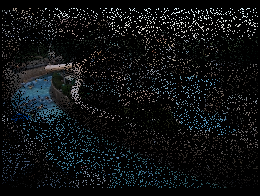
\includegraphics[width=1.25cm]{figures/input.png}};
        \node[] at (-4.6, 0.4) {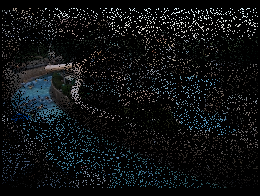
\includegraphics[width=1.25cm]{figures/input.png}};
        \node[] at (-4.7, 0.3) {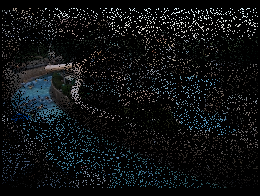
\includegraphics[width=1.25cm]{figures/input.png}};
        \node[] at (-4.8, 0.2) {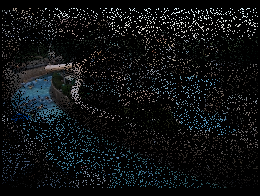
\includegraphics[width=1.25cm]{figures/input.png}};
        \node[] at (-4.9, 0.1) {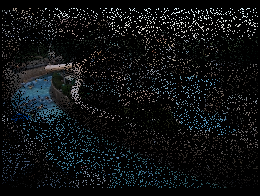
\includegraphics[width=1.25cm]{figures/input.png}};
        \node[] at (-5, 0) {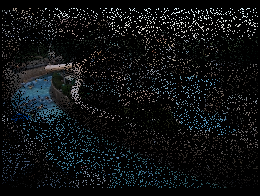
\includegraphics[width=1.25cm]{figures/input.png}};
        \node[] at (-5, 2.75) {Fovea sampled input sequence};
        \draw[->, very thick, black] (-1.5, 0) -- node[midway, above, text width=3cm] {Reconstruction \& Super-Resolution} (1.0, 0);
        \node[] at (4.5, 0.5) {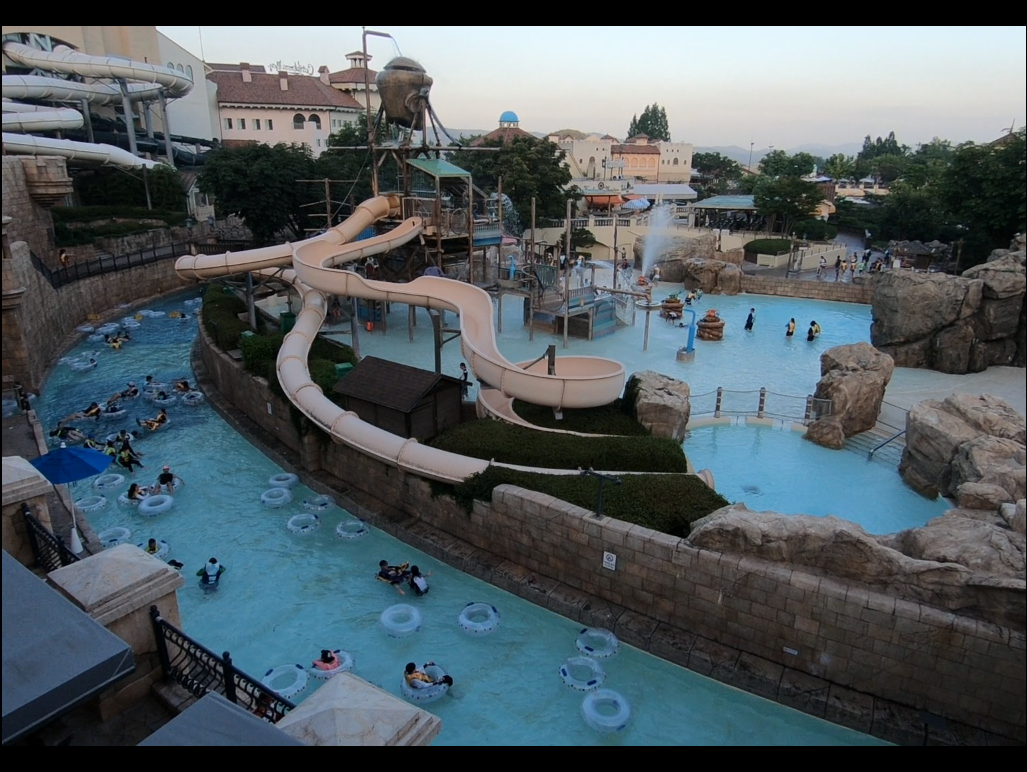
\includegraphics[width=5cm]{figures/label.png}};
        \node[] at (4.4, 0.4) {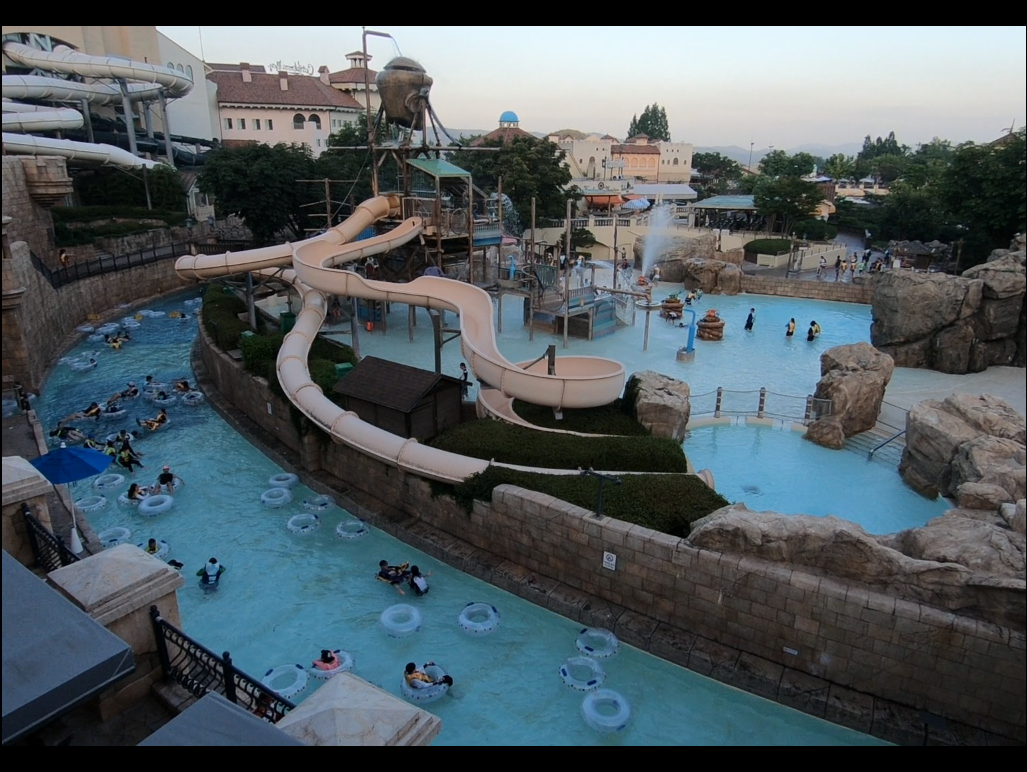
\includegraphics[width=5cm]{figures/label.png}};
        \node[] at (4.3, 0.3) {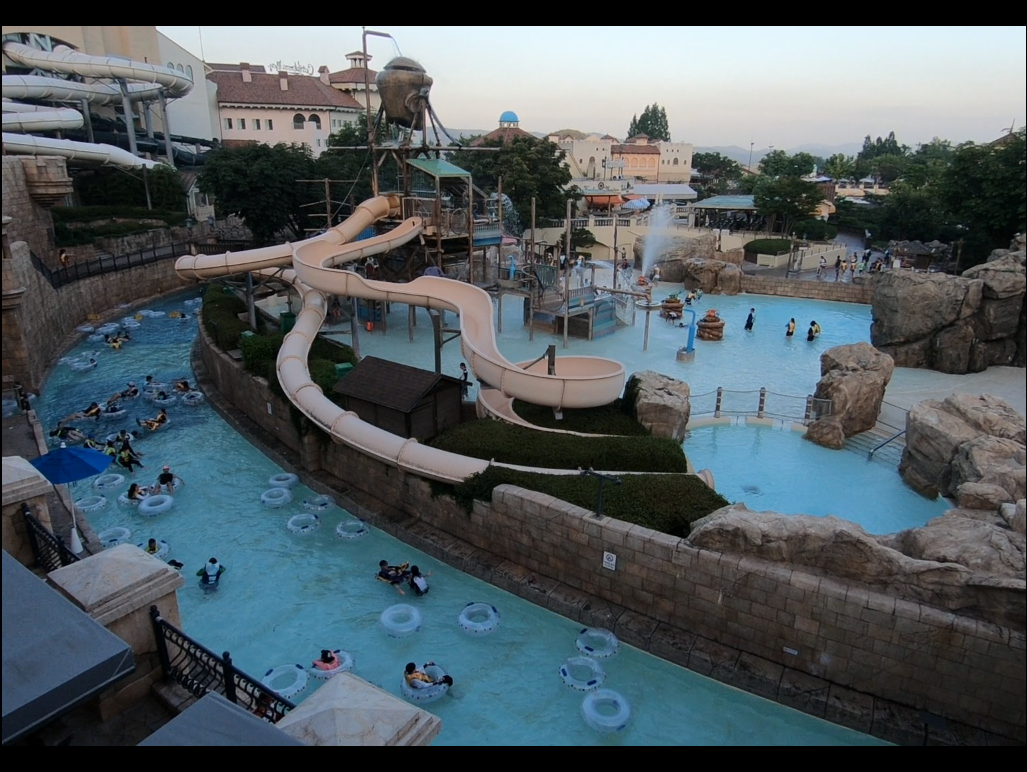
\includegraphics[width=5cm]{figures/label.png}};
        \node[] at (4.2, 0.2) {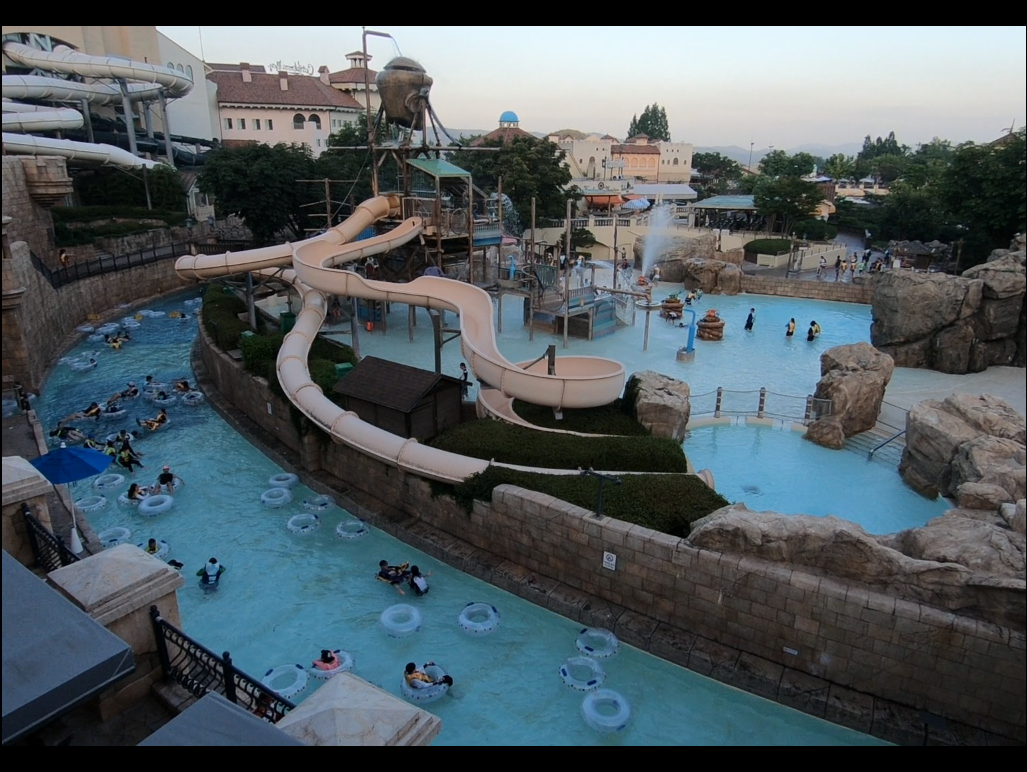
\includegraphics[width=5cm]{figures/label.png}};
        \node[] at (4.1, 0.1) {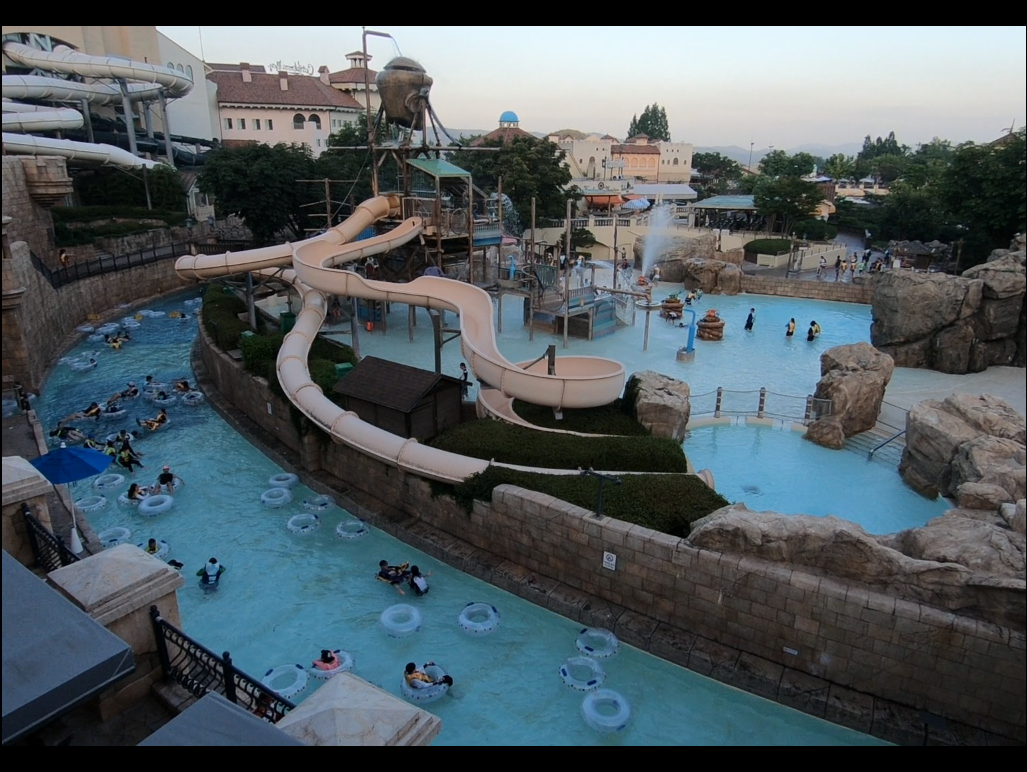
\includegraphics[width=5cm]{figures/label.png}};
        \node[] at (4.0, 0) {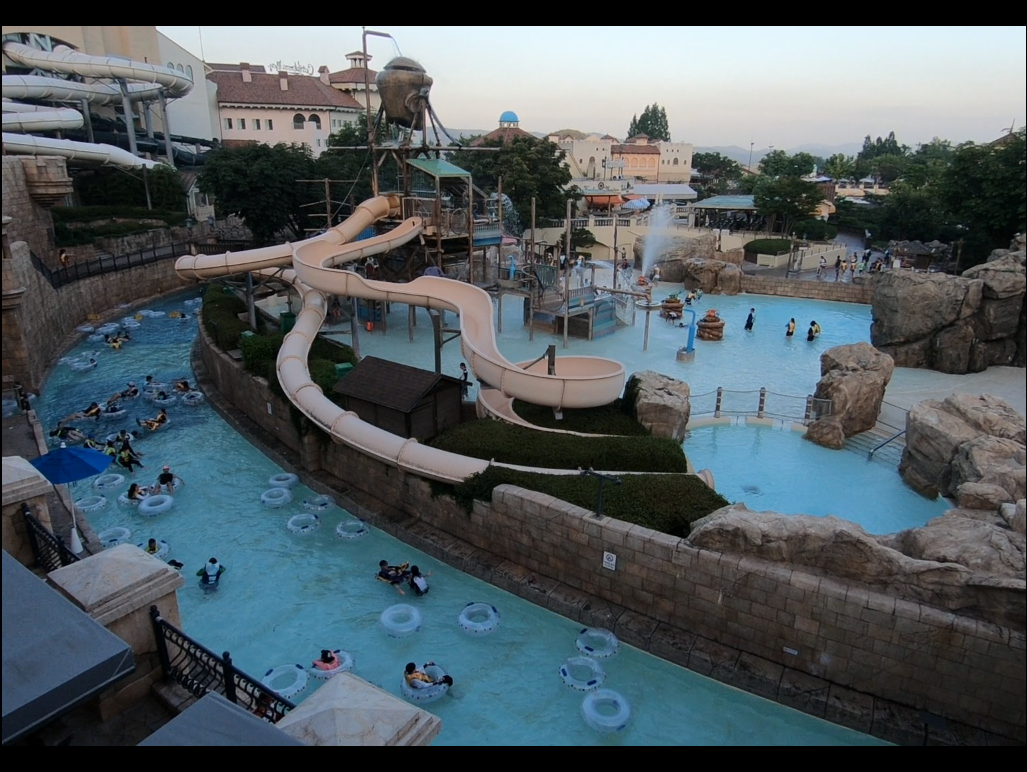
\includegraphics[width=5cm]{figures/label.png}};
        \node[] at (4.4, 2.75) {Reconstructed \& upsampled sequence};
    \end{tikzpicture}
\end{center}}

\only<2>{
\begin{center}
    \begin{tikzpicture}[>={Stealth[inset=0pt,length=10pt,angle'=45]}]
        \node[] at (-4.5, 0.5) {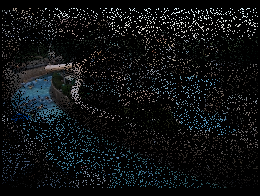
\includegraphics[width=5cm]{figures/input.png}};
        \node[] at (-4.6, 0.4) {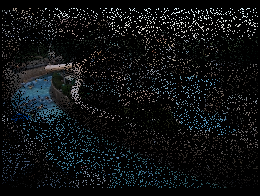
\includegraphics[width=5cm]{figures/input.png}};
        \node[] at (-4.7, 0.3) {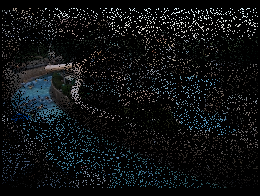
\includegraphics[width=5cm]{figures/input.png}};
        \node[] at (-4.8, 0.2) {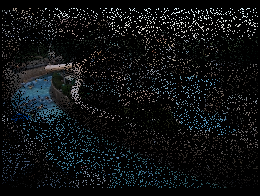
\includegraphics[width=5cm]{figures/input.png}};
        \node[] at (-4.9, 0.1) {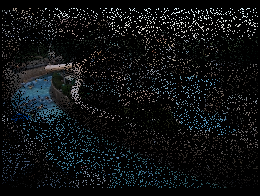
\includegraphics[width=5cm]{figures/input.png}};
        \node[] at (-5, 0) {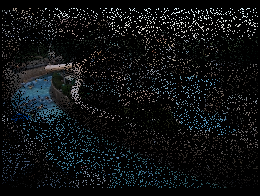
\includegraphics[width=5cm]{figures/input.png}};
        \node[] at (-5, 2.75) {Fovea sampled input sequence};
        \draw[->, very thick, black] (-1.5, 0) -- node[midway, above, text width=3cm] {Reconstruction \& Super-Resolution} (1.0, 0);
        \node[] at (4.5, 0.5) {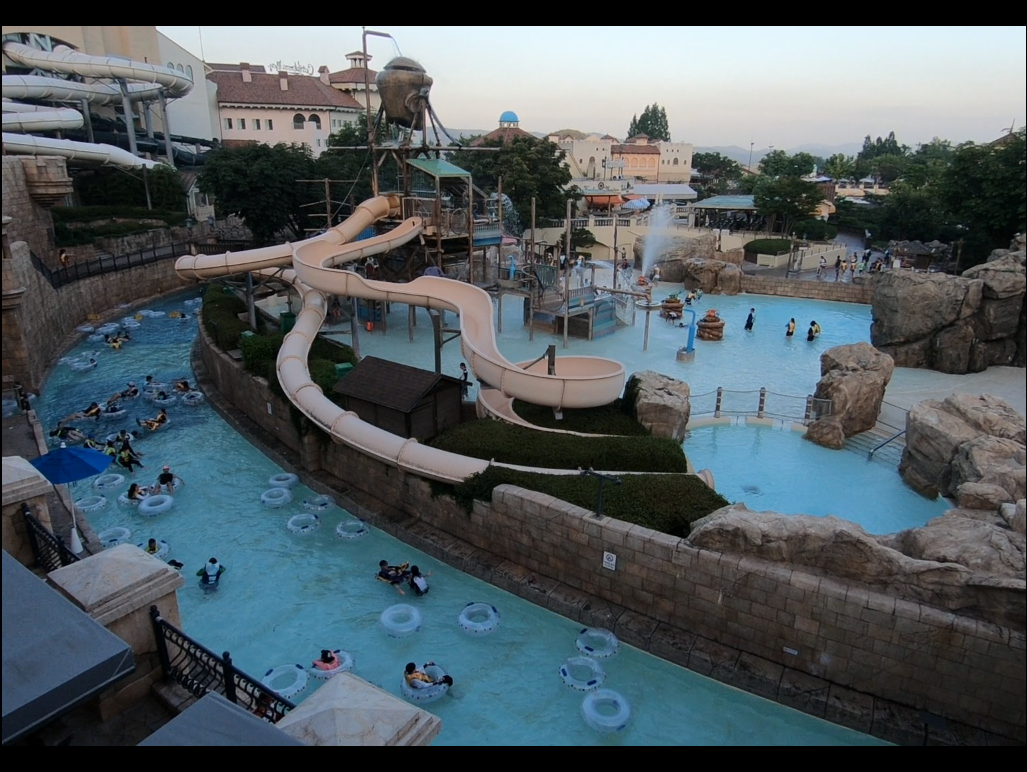
\includegraphics[width=5cm]{figures/label.png}};
        \node[] at (4.4, 0.4) {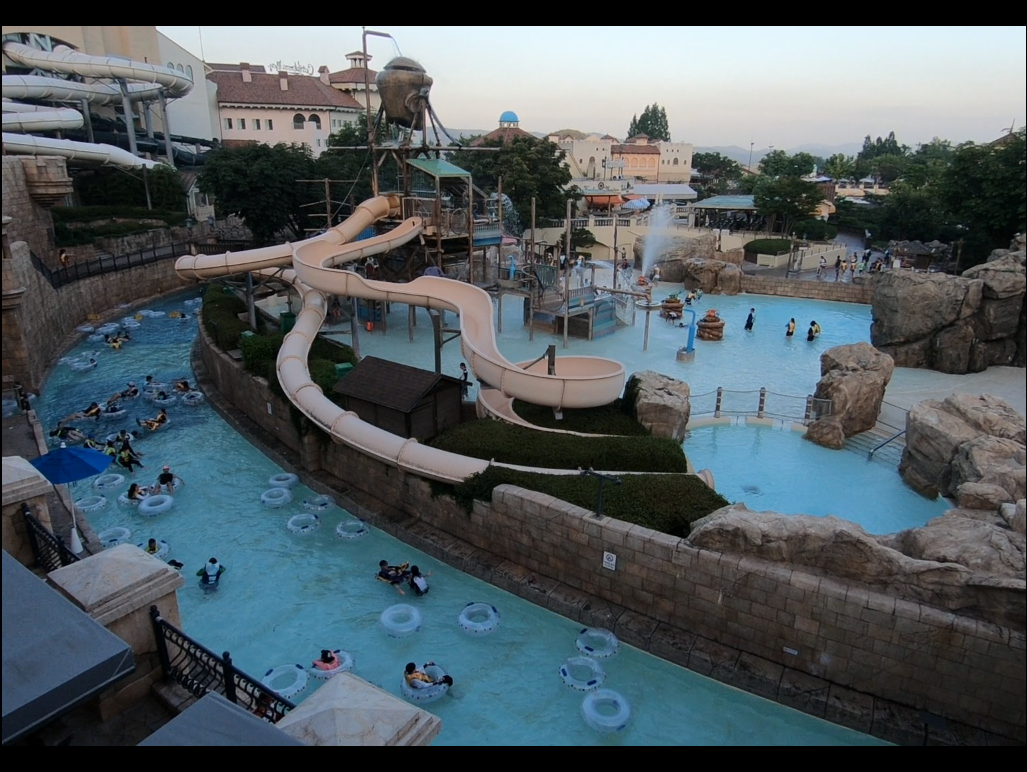
\includegraphics[width=5cm]{figures/label.png}};
        \node[] at (4.3, 0.3) {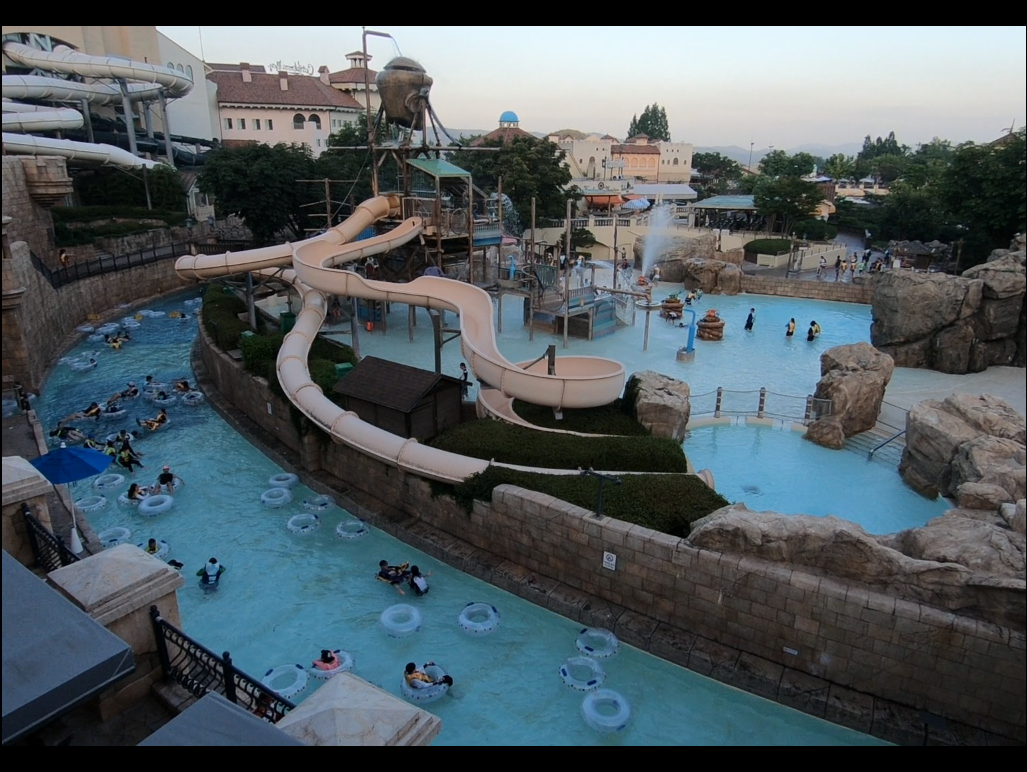
\includegraphics[width=5cm]{figures/label.png}};
        \node[] at (4.2, 0.2) {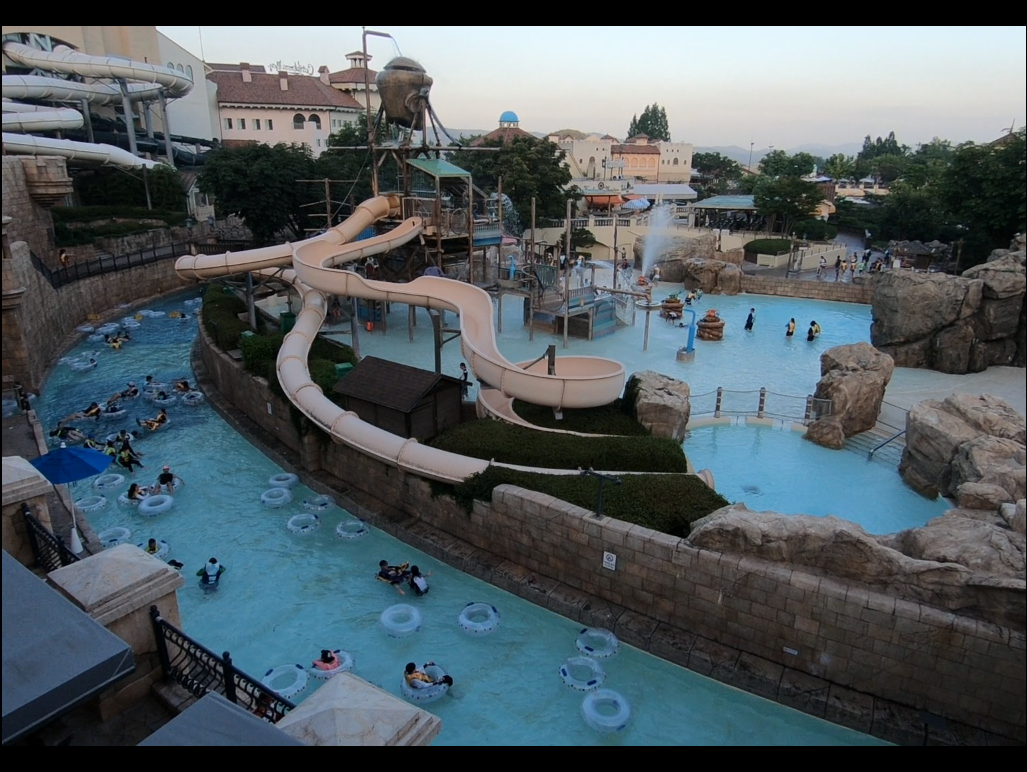
\includegraphics[width=5cm]{figures/label.png}};
        \node[] at (4.1, 0.1) {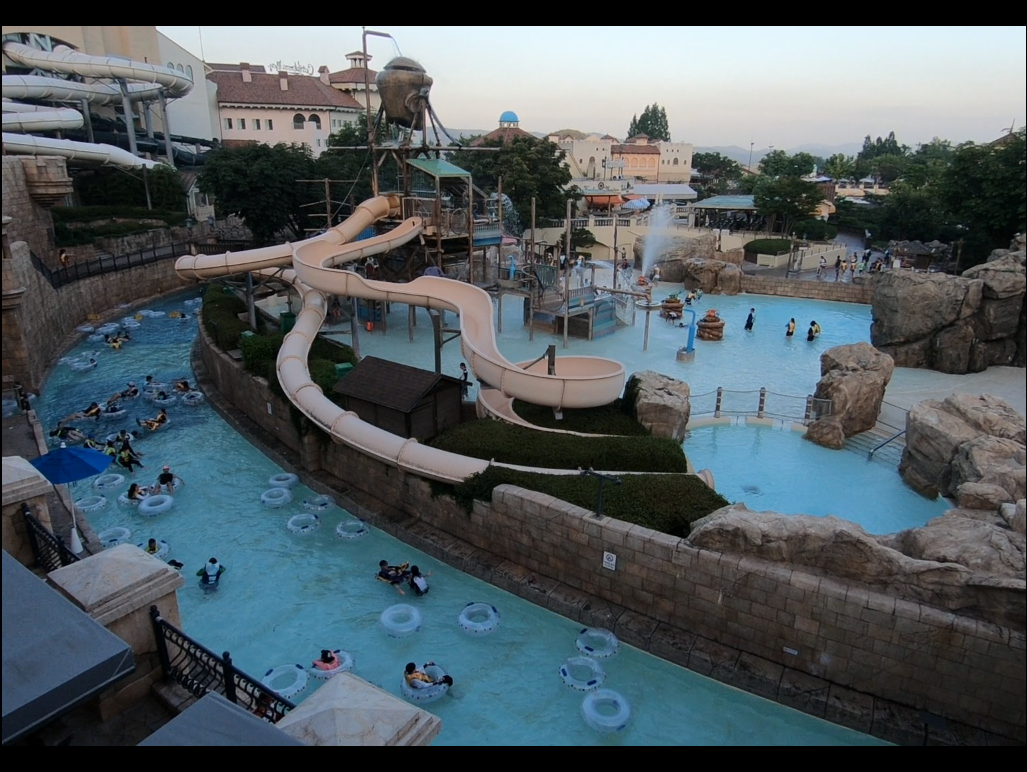
\includegraphics[width=5cm]{figures/label.png}};
        \node[] at (4.0, 0) {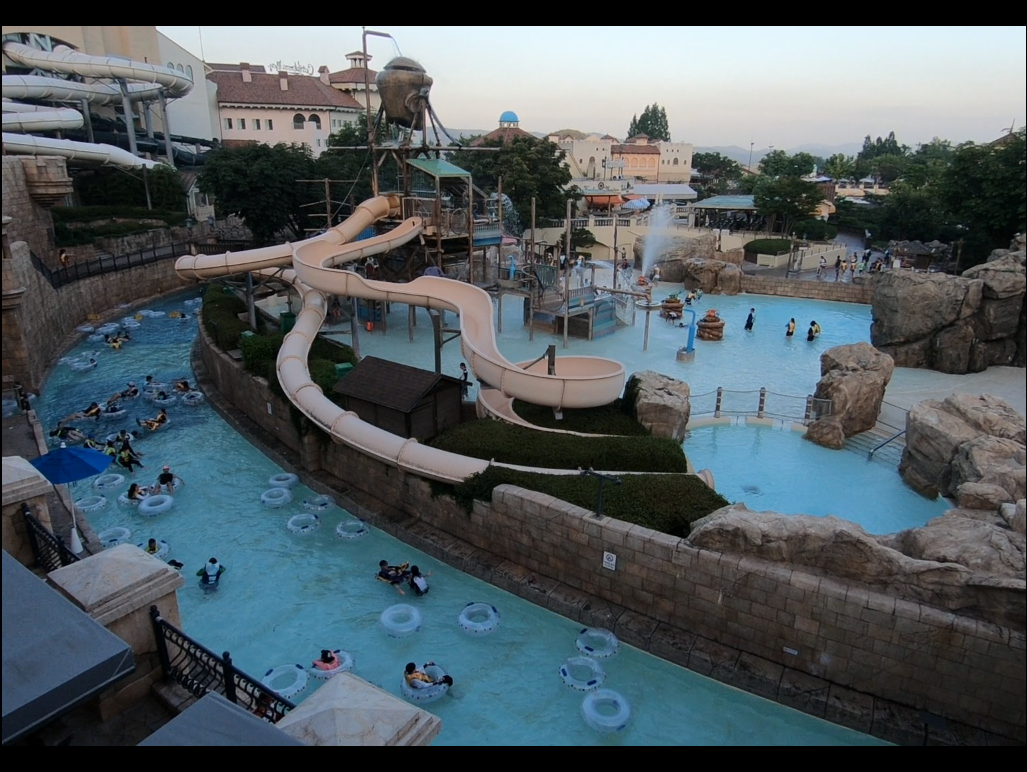
\includegraphics[width=5cm]{figures/label.png}};
        \node[] at (4.4, 2.75) {Reconstructed \& upsampled sequence};
    \end{tikzpicture}
\end{center}}
\end{frame}

%%%%%%%%% Related Work %%%%%%%%%

\begin{frame}{Fovea sample reconstruction}
\framesubtitle{Related Work}
\textbf{DeepFovea} - \citet{deepfovea} (Facebook AI)
\begin{itemize}
    \item Reconstructions of most plausible peripheral video from small portion of pixels in each frame
    \item Able to reconstruct video sequences (128 $\times$ 128)
    \item Recurrent U-Net reconstruction network
    \item Loss combination (adversarial, perceptual, optical flow)
\end{itemize}
\end{frame}

\begin{comment}
\begin{frame}{Fovea sample reconstruction}
\framesubtitle{Related Work}
\textbf{Classic Convolution}
\begin{itemize}
    \item Fixed sampling locations
\end{itemize}

\textbf{Deformable Convolutions}
\begin{itemize}
    \item v1: learns offset to original sampling location with seperate traditional convolution \cite{deformableconv1}
    \item v2: also learns additional modulation mechanism \cite{deformableconv}
    \item Performance benefits in multiple use cases (e.g. semantic segmentation, object detection)
\end{itemize}
\end{frame}
\end{comment}

\begin{frame}{Video Super-Resolution}
\framesubtitle{Related Work}
\textbf{Detail-revealing deep video super-resolution} - \citet{valillasuperres} (\citeyear{valillasuperres})
\begin{itemize}
    \item Sub-pixel motion compensation layers (improved frame alignment)
\end{itemize}

\vspace{0.5cm}

\textbf{Video restoration with enhanced deformable convolutional networks} - \citet{deformablesuperres} (\citeyear{deformablesuperres})
\begin{itemize}
    \item Enhanced deformable convolution (frame alignment, temporal and spatial attention)
\end{itemize}

\vspace{0.5cm}

\pause

\textbf{Additional Work}
\begin{itemize}
    \item Video super-resolution with convolutional neural networks - \citet{videosuperrescnn} (\citeyear{videosuperrescnn})
    \item Video super-resolution via deep draft-ensemble learning - \citet{videosuperresdraft} (\citeyear{videosuperresdraft})
    \item Dictionary-based multiple frame video super-resolution - \citet{videosuperresdict} (\citeyear{videosuperresdict})
\end{itemize}
\end{frame}

%%%%%%%%% Method %%%%%%%%%

\begin{frame}{Reconstruction Model Architecture}
\framesubtitle{Method}
\vspace{1cm}
\begin{figure}[h!]
    \centering
    \begin{tikzpicture}[xscale=0.6, yscale=0.6, every node/.style={scale=0.625}, >={Stealth[inset=0pt,length=2.8pt,angle'=45]}]
	% Residual enocder block
	\begin{scope}[shift={(0.0,0)}]
		\draw[white, fill=tud0a] (0,-0.5) rectangle++(4.5,5.5);
		\node at (2.25,4.5) {Residual encoder block};
		\draw[tud1c, thick,  ->] (0,2) -- (0.5,2);
		\draw[black, fill=tud2b] (0.5,0.5) rectangle++(0.5,3);
		\node[rotate=90] at (0.75,2) {$3\times 3$ Convolution};
		\draw[tud1c, thick,  ->] (1,2) -- (2,2);
		\draw[black, fill=white] (1.46,2) circle [radius=0.15] node {\begin{tikzpicture}\draw[tud9b] (-0.1, -0.12) -- (0.0, -0.1) -- (0.1, 0.0);\end{tikzpicture}};
		\draw[black, fill=tud2b] (2,0.5) rectangle++(0.5,3);
		\node[rotate=90] at (2.25,2) {$3\times 3$ Convolution};
		\draw[tud1c, thick,  ->] (2.5,2) -- (3.5,2);
		\draw[black, fill=white] (2.73,2) circle [radius=0.15] node {\begin{tikzpicture}\draw[tud9b] (-0.1, -0.12) -- (0.0, -0.1) -- (0.1, 0.0);\end{tikzpicture}};
		\draw[black, fill=white] (3.1,2) circle [radius=0.15] node {$+$};
		\draw[tud1c, thick,  ->] (0.25,2) -- (0.25,0) -- (3.1,0) -- (3.1,1.85);
		\draw[black, fill=tud2b] (3.5,0.5) -- (3.5,3.5) -- (4,3) -- (4,1) -- (3.5,0.5);
		\node[rotate=90] at (3.75,2) {Average pool};
		\draw[tud1c, thick,  ->] (4,2) -- (4.5,2);
	\end{scope}
    
    % Network
    \begin{scope}[shift={(4.6, 2.0)}, xscale=0.625, yscale=0.625]
        \draw[tud1c, thick, ->] (0.0, 0.0) -- (0.5, 0.0);
    	\draw[black, fill=tud0a] (0.5, -3.0) rectangle++ (1.0, 6.0);
    	\node[rotate=90] at (1.0, 0.0) {Res block 1};
    	
    	\draw[tud1c, thick, ->] (1.5, 0.0) -- (2.5, 0.0);
    	\draw[black, fill=tud0a] (2.5, -2.5) rectangle++ (1.0, 5.0);
    	\node[rotate=90] at (3.0, 0.0) {Res block 2};
    	
    	\draw[tud1c, thick, ->] (3.5, 0.0) -- (4.5, 0.0);
    	\draw[black, fill=tud0a] (4.5, -2.0) rectangle++ (1.0, 4.0);
    	\node[rotate=90] at (5.0, 0.0) {Res block 3};
    	
    	\draw[tud1c, thick, ->] (5.5, 0.0) -- (6.5, 0.0);
    	\draw[black, fill=tud0a] (6.5, -1.5) rectangle++ (1.0, 3.0);
    	\node[rotate=90] at (7.0, 0.0) {\small{Res block 4}};	
    	
    	\draw[tud1c, thick, ->] (7.5, 0.0) -- (8.5, 0.0);
    	\draw[black, fill=tud0a] (8.5, -1.0) rectangle++ (1.0, 2.0);
    	\node[rotate=90] at (9.0, 0.0) {\tiny{Res block 5}};
    	
    	\draw[tud1c, thick, ->] (9.5, 0.0) -- (10.5, 0.0);
    	\draw[black, fill=white] (10.0, 0.0) circle [radius=0.2] node {\tiny{c.}};
    	\draw[tud8c, thick, ->] (10.0, 4.5) -- (10.0, 0.25);
    	\draw[black, fill=tud7c!20] (10.5, -1.5) rectangle++ (1.0, 3.0);
    	\node[rotate=90] at (11.0, 0.0) {\tiny{Temp block 1}};
    	\draw[tud8c, thick, ->] (10.5, -1.5) |- (10.0, -2.0) -- (10.0, -4.5);
    	
    	\draw[tud1c, thick, ->] (11.5, 0.0) -- (12.5, 0.0);
    	\draw[black, fill=white] (12.0, 0.0) circle [radius=0.2] node {\tiny{c.}};
    	\draw[tud8c, thick, ->] (12.0, 4.5) -- (12.0, 0.2);
    	\draw[black, fill=tud7c!20] (12.5, -2.0) rectangle++ (1.0, 4.0);
    	\node[rotate=90] at (13.0, 0.0) {\small{Temp block 2}};
    	\draw[tud8c, thick, ->] (12.5, -2.0) |- (12.0, -2.5) -- (12.0, -4.5);
    	
    	\draw[tud1c, thick, ->] (13.5, 0.0) -- (14.5, 0.0);
    	\draw[black, fill=white] (14.0, 0.0) circle [radius=0.2] node {\tiny{c.}};
    	\draw[tud8c, thick, ->] (14.0, 4.5) -- (14.0, 0.25);
    	\draw[black, fill=tud7c!20] (14.5, -2.5) rectangle++ (1.0, 5.0);
    	\node[rotate=90] at (15.0, 0.0) {Temp block 3};
    	\draw[tud8c, thick, ->] (14.5, -2.5) |- (14.0, -3.0) -- (14.0, -4.5);
    	
    	\draw[tud1c, thick, ->] (15.5, 0.0) -- (16.5, 0.0);
    	\draw[black, fill=white] (16.0, 0.0) circle [radius=0.2] node {\tiny{c.}};
    	\draw[tud8c, thick, ->] (16.0, 4.5) -- (16.0, 0.25);
    	\draw[black, fill=tud7c!20] (16.5, -3.0) rectangle++ (1.0, 6.0);
    	\node[rotate=90] at (17.0, 0.0) {Temp block 4};
    	\draw[tud8c, thick, ->] (16.5, -3.0) |- (16.0, -3.5) -- (16.0, -4.5);
    	
    	\draw[tud1c, thick, ->] (17.5, 0.0) -- (18.5, 0.0);
    	\draw[black, fill=tud10a!20] (18.5, -3.5) rectangle++ (1.0, 7.0);
    	\node[rotate=90] at (19.0, 0.0) {Super-resolution block 1};
	
    	\draw[tud1c, thick, ->] (19.5, 0.0) -- (20.5, 0.0);
    	\draw[black, fill=tud10a!20] (20.5, -4.0) rectangle++ (1.0, 8.0);
    	\node[rotate=90] at (21.0, 0.0) {Super-resolution block 2};
    	   
    	\draw[densely dashdotted, tud8c, thick, ->] (22.0, 4.5) -- (22.0, -4.5);
    	\node[black, rotate=90] at (22.35, 0.0) {Time};
    	
    	\draw[densely dashdotted, tud0c, thick, ->] (7.5,-1.5) .. controls (8.5,-2) and (9.5,-2) .. (10.5,-1.5);
    	\draw[densely dashdotted, tud0c, thick, ->] (5.5,-2) .. controls (7.5,-2.5) and (10.5,-2.5) .. (12.5,-2);
    	\draw[densely dashdotted, tud0c, thick, ->] (3.5,-2.5) .. controls (5.5,-3) and (12.5,-3) .. (14.5,-2.5);
    	\draw[densely dashdotted, tud0c, thick, ->] (1.5,-3) .. controls (3.5,-3.5) and (14.5,-3.5) .. (16.5,-3);
    \end{scope}
    
	% Temporal block
	\begin{scope}[shift={(19.0,0)}]
		\draw[white, fill=tud7c!20] (0.0, -0.5) rectangle++ (4.5, 5.5);
		\node at (2.25, 4.5) {Temporal decoder block};
		\draw[tud1c, thick,  ->] (0.0, 2.0) -- (0.5, 2.0);
		\draw[black, fill=tud2b] (0.5, 0.5) rectangle++ (0.5, 3.0);
		\node[rotate=90] at (0.75, 2.0) {$3\times 3$ Convolution};
		\draw[tud1c, thick,  ->] (1.0, 2.0) -- (2.0, 2.0);
		\draw[black, fill=tud2b] (1.1, 1.5) rectangle++ (0.25, 1.0);
		\node[rotate=90] at (1.225, 2.0) {\tiny{Norm.}};
    	\draw[tud8c, thick, ->] (1.6, 2.0) -- (1.6, -0.5);
		\draw[black, fill=white] (1.6,2.0) circle [radius=0.15] node {\begin{tikzpicture}\draw[tud9b] (-0.1, -0.12) -- (0.0, -0.1) -- (0.1, 0.0);\end{tikzpicture}};
		\draw[black, fill=tud2b] (2.0, 0.5) rectangle++ (0.5, 3.0);
		\node[rotate=90] at (2.25, 2.0) {$3\times 3$ Convolution};
		\draw[tud1c, thick,  ->] (2.5, 2.0) -- (3.5, 2.0);
		\draw[black, fill=white] (2.73,2) circle [radius=0.15] node {\begin{tikzpicture}\draw[tud9b] (-0.1, -0.12) -- (0.0, -0.1) -- (0.1, 0.0);\end{tikzpicture}};
		\draw[black, fill=white] (3.1,2) circle [radius=0.15] node {$+$};
		\draw[tud1c, thick,  ->] (0.25, 2.0) -- (0.25, 0.0) -- (3.1,0) -- (3.1, 1.85);
		\draw[black, fill=tud2b] (3.5, 0.5) -- (3.5, 3.5) -- (4.0, 4.0) -- (4.0, 0.0) -- (3.5, 0.5);
		\node[rotate=90] at (3.75, 2.0) {Bilinear upsample};
		\draw[tud1c, thick,  ->] (4.0, 2.0) -- (4.5, 2.0);
	\end{scope}
	
	\begin{scope}[shift={(23.7, 0)}]
	    \draw[white, fill=tud10a!20] (0.0, -0.5) rectangle++ (5.25, 5.5);
    	\node at (2.625, 4.5) {Super-resolution block};
    	\draw[tud1c, thick,  ->] (0.0, 2.0) -- (0.5, 2.0);
    	\draw[black, fill=tud2b] (0.5, 0.5) rectangle++ (0.5, 3.0);
    	\node[rotate=90] at (0.75, 2.0) {$3\times 3$ D. Conv.};
    	\draw[tud1c, thick,  ->] (1.0, 2.0) -- (1.75,2);
    	\draw[black, fill=white] (1.3,2.0) circle [radius=0.15] node {\begin{tikzpicture}\draw[tud9b] (-0.1, -0.12) -- (0.0, -0.1) -- (0.1, 0.0);\end{tikzpicture}};
    	\draw[black, fill=tud2b] (1.75,0.5) -- (1.75,3.5) -- (2.25,4) -- (2.25,0) -- (1.75,0.5);
    	\node[rotate=90] at (2,2) {Bilinear upsample};
    	\draw[tud1c, thick,  ->] (2.25, 2.0) -- (2.75,2);
    	\draw[black, fill=tud2b] (2.75, 0.5) rectangle++ (0.5, 3.0);
    	\node[rotate=90] at (3.0, 2.0) {$3\times 3$ D. Conv.};
    	\draw[tud1c, thick,  ->] (3.25, 2.0) -- (4.25,2);
    	\draw[black, fill=white] (3.5,2.0) circle [radius=0.15] node {\begin{tikzpicture}\draw[tud9b] (-0.1, -0.12) -- (0.0, -0.1) -- (0.1, 0.0);\end{tikzpicture}};
		\draw[black, fill=white] (3.85,2) circle [radius=0.15] node {$+$};
		\draw[tud1c, thick,  ->] (0.25, 2.0) -- (0.25, -0.25) -- (3.85,-0.25) -- (3.85, 1.85);
		\draw[black, fill=tud2b] (4.25, 0.5) rectangle++ (0.5, 3.0);
    	\node[rotate=90] at (4.5, 2.0) {$1\times 1$ D. Conv.};
		\draw[tud1c, thick,  ->] (4.75, 2.0) -- (5.25, 2.0);
	\end{scope}
\end{tikzpicture}

















    \caption{Architecture of the reconstruction network.}
    \label{fig:reconstructionnetwork}
\end{figure}
\end{frame}

\begin{frame}{Training process}
\framesubtitle{Method}
\textbf{Loss function}
\begin{equation}
    \mathcal{L}=w_{\text{sv}}\,\mathcal{L}_{\text{sv}} + w_{\text{adv}}\,\mathcal{L}_{\text{adv}} + w_{\text{adv fft}}\,\mathcal{L}_{\text{adv fft}} + w_{\text{flow}}\,\mathcal{L}_{\text{flow}} + w_{\text{LPIPS}}\,\mathcal{L}_{\text{LPIPS}}
\end{equation}
\pause
\begin{itemize}
    \item Supervised loss (general and adaptive robust loss function - \citet{adaptiveroubustloss}) $\quad\mathcal{L}_{\text{sv}}=p(x,\alpha,c)+\log Z(\alpha),\;\; p(x=\sum_{i\in(c\,h\,w)}\hat{\Tensor{I}}-\Tensor{I},\alpha,c)=\frac{\abs{\alpha -2}}{\alpha}\left(\left(\frac{\left(x/c\right)^2}{\abs{\alpha-2}}+1\right)^{(\alpha/2)}-1\right)$
    \item Adversarial loss \cite{gan} $\quad\quad\,\mathcal{L}_{\text{adv, adv fft}}=-\Mean{\log\left(\operatorname{D}\left(\hat{\Tensor{I}}\right)\right)}$
    \item Optical flow loss \cite{pwcnet, deepfovea} $\quad\mathcal{L}_{\text{flow}}=\frac{1}{5}\sum_{i=1}^{5}\frac{1}{c_{\text{rgb}}\,h_{i}\,w_{i}}\norm{\hat{\Tensor{I}}_{i}-\operatorname{Warp}\left[\hat{\Tensor{I}}_{i+1}\right]}_{1}$
    \item Perceptual loss \cite{perceptual} $\quad\quad\;\mathcal{L}_{\text{LPIPS}} = \frac{1}{5}\sum_{i=1}^{5}\frac{1}{b\,c_{i}\,h_{i}\,w_{i}}\norm{\operatorname{VGG}_{i,2}\left(\hat{\Tensor{I}}\right) - \operatorname{VGG}_{i,2}\left(\Tensor{I}\right)}_{1}$
\end{itemize}
\end{frame}

\begin{frame}{Discriminator Architecture}
\framesubtitle{Method}
    \vspace{0.5cm}
    \begin{figure}
        \centering
        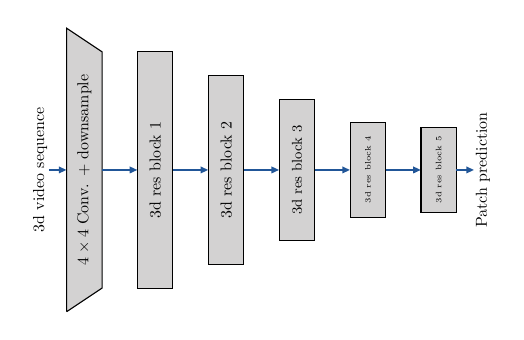
\begin{tikzpicture}[xscale=0.6, yscale=0.75, every node/.style={scale=0.575}, >={Stealth[inset=0pt,length=2.8pt,angle'=45]}]
    \begin{scope}[xscale=0.75, yscale=0.8]
    	\node[rotate=90] at (-0.25, 0.0) {3d video sequence};
    	\draw[tud1c, thick, ->] (0.0, 0.0) -- (0.5, 0.0);
        \draw[black, fill=tud0a] (0.5, -3.0) -- (0.5, 3.0) -- (1.5, 2.5) -- (1.5, -2.5) -- (0.5, -3.0);
        \node[rotate=90] at (1.0, 0.0) {$4 \times 4$ Conv. + downsample};
    	
    	\draw[tud1c, thick, ->] (1.5, 0.0) -- (2.5, 0.0);
    	\draw[black, fill=tud0a] (2.5, -2.5) rectangle++ (1.0, 5.0);
    	\node[rotate=90] at (3.0, 0.0) {3d res block 1};
    	
    	\draw[tud1c, thick, ->] (3.5, 0.0) -- (4.5, 0.0);
    	\draw[black, fill=tud0a] (4.5, -2.0) rectangle++ (1.0, 4.0);
    	\node[rotate=90] at (5.0, 0.0) {3d res block 2};
    	
    	\draw[tud1c, thick, ->] (5.5, 0.0) -- (6.5, 0.0);
    	\draw[black, fill=tud0a] (6.5, -1.5) rectangle++ (1.0, 3.0);
    	\node[rotate=90] at (7.0, 0.0) {\small{3d res block 3}};
    	
    	\draw[tud1c, thick, ->] (7.5, 0.0) -- (8.5, 0.0);
    	\draw[black, fill=tud0a] (8.5, -1.0) rectangle++ (1.0, 2.0);
    	\node[rotate=90] at (9.0, 0.0) {\tiny{3d res block 4}};
    
    	\draw[tud1c, thick, ->] (9.5, 0.0) -- (10.5, 0.0);
    	\draw[black, fill=tud0a] (10.5, -0.9) rectangle++ (1.0, 1.8);
    	\node[rotate=90] at (11.0, 0.0) {\tiny{3d res block 5}};
    	
    	\draw[tud1c, thick, ->] (11.5, 0.0) -- (12.0, 0.0);
    	\node[rotate=90] at (12.25, 0.0) {Patch prediction};
	\end{scope}
\end{tikzpicture}\hspace{1.0cm}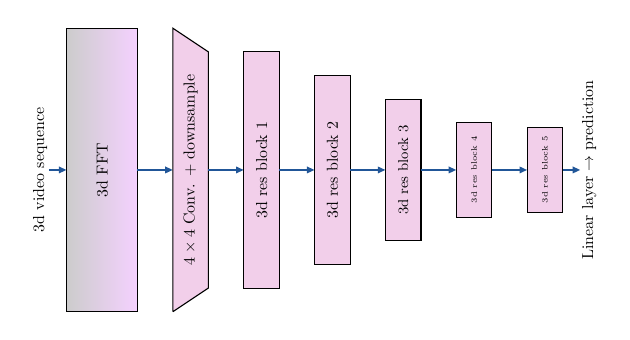
\begin{tikzpicture}[xscale=0.6, yscale=0.75, every node/.style={scale=0.575}, >={Stealth[inset=0pt,length=2.8pt,angle'=45]}]
    \begin{scope}[xscale=0.75, yscale=0.8]
    	\node[rotate=90] at (-3.25, 0.0) {3d video sequence};
    	\draw[tud1c, thick, ->] (-3.0, 0.0) -- (-2.5, 0.0);
    	\shade[black, left color=tud0a, right color=tud10a!20] (-2.5, -3.0) rectangle++ (2.0, 6.0);
    	\draw[black] (-2.5, -3.0) rectangle++ (2.0, 6.0);
        \node[rotate=90] at (-1.5, 0.0) {3d FFT};
    	\draw[tud1c, thick, ->] (-0.5, 0.0) -- (0.5, 0.0);
        \draw[black, fill=tud10a!20] (0.5, -3.0) -- (0.5, 3.0) -- (1.5, 2.5) -- (1.5, -2.5) -- (0.5, -3.0);
        \node[rotate=90] at (1.0, 0.0) {$4 \times 4$ Conv. + downsample};
    	
    	\draw[tud1c, thick, ->] (1.5, 0.0) -- (2.5, 0.0);
    	\draw[black, fill=tud10a!20] (2.5, -2.5) rectangle++ (1.0, 5.0);
    	\node[rotate=90] at (3.0, 0.0) {3d res block 1};
    	
    	\draw[tud1c, thick, ->] (3.5, 0.0) -- (4.5, 0.0);
    	\draw[black, fill=tud10a!20] (4.5, -2.0) rectangle++ (1.0, 4.0);
    	\node[rotate=90] at (5.0, 0.0) {3d res block 2};
    	
    	\draw[tud1c, thick, ->] (5.5, 0.0) -- (6.5, 0.0);
    	\draw[black, fill=tud10a!20] (6.5, -1.5) rectangle++ (1.0, 3.0);
    	\node[rotate=90] at (7.0, 0.0) {\small{3d res block 3}};
    	
    	\draw[tud1c, thick, ->] (7.5, 0.0) -- (8.5, 0.0);
    	\draw[black, fill=tud10a!20] (8.5, -1.0) rectangle++ (1.0, 2.0);
    	\node[rotate=90] at (9.0, 0.0) {\tiny{3d res block 4}};
    
    	\draw[tud1c, thick, ->] (9.5, 0.0) -- (10.5, 0.0);
    	\draw[black, fill=tud10a!20] (10.5, -0.9) rectangle++ (1.0, 1.8);
    	\node[rotate=90] at (11.0, 0.0) {\tiny{3d res block 5}};
    	
    	\draw[tud1c, thick, ->] (11.5, 0.0) -- (12.0, 0.0);
    	\node[rotate=90] at (12.25, 0.0) {Linear layer $\rightarrow$ prediction};
	\end{scope}
\end{tikzpicture}
        \caption{Discriminator network on the left and FFT discriminator network on the right.}
        \label{fig:discriminatornetorks}
    \end{figure}
\end{frame}

\begin{frame}{Dataset and Fovea Sampling}
\framesubtitle{Method}
\textbf{REDS dataset} - \citet{REDS}
\begin{itemize}
    \item 300 sequences of 100 high-quality natural RGB video frames each
    \item Resolution 720 $\times$ 1280
\end{itemize}
\textbf{Fovea Sampling}
\begin{itemize}
    \item Low chance of pixels not being masked out in or closer to focus point
    \item Higher chance of being masked out moving away from focus point
    \item Mask generated on downsampled image (relates to approximately 19\% of the information in the low-res image and to \textbf{1.1\%} of pixels compared to the high-res image)
\end{itemize}
\end{frame}

%%%%%%%%% Results %%%%%%%%%
\begin{frame}{Results}
    \framesubtitle{Qualitative results - with and without reset}
    \begin{center}
    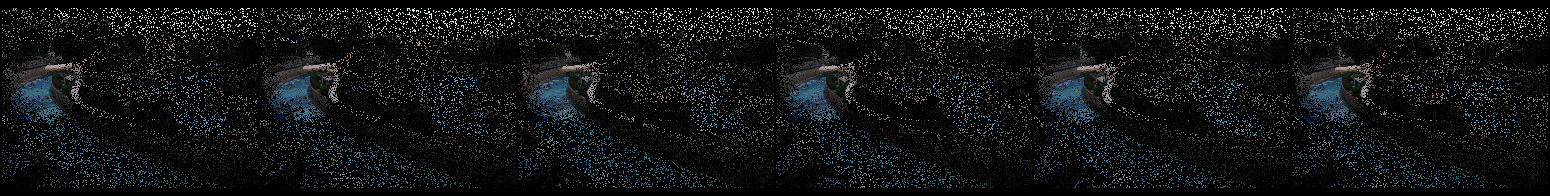
\includegraphics[width=0.75\linewidth]{figures/reset/input_220_2020-05-04 11_17_59.593499.png}
    \includegraphics[width=0.75\linewidth]{figures/reset/prediction_220_2020-05-04 11_17_55.343509.png}
    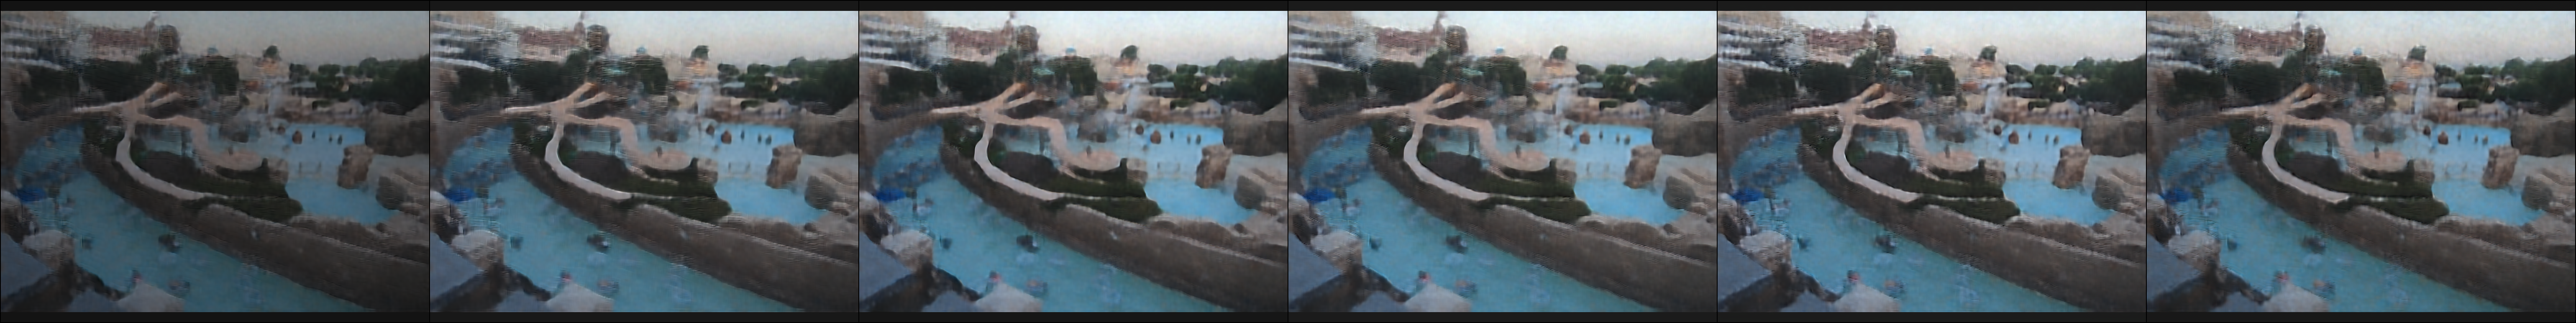
\includegraphics[width=0.75\linewidth]{figures/no_rest/prediction_220_2020-05-06 09_57_18.378952.png}
    \includegraphics[width=0.75\linewidth]{figures/reset/label_220_2020-05-04 11_17_57.695080.png}
    \end{center}
\end{frame}

\begin{frame}{Results}
    \framesubtitle{Qualitative results - with and without reset}
    \begin{center}
    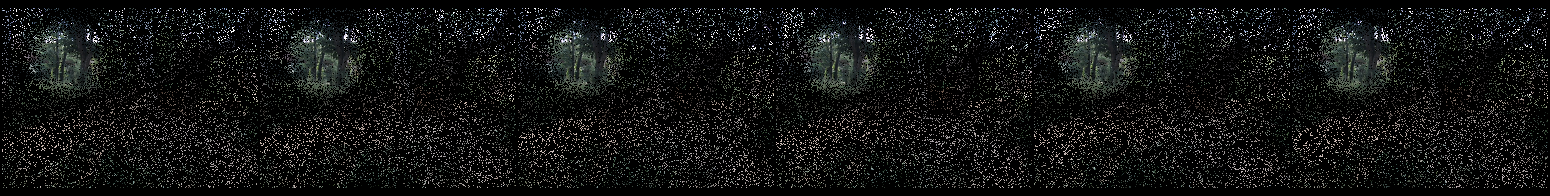
\includegraphics[width=0.75\linewidth]{figures/reset/input_432_2020-05-04 11_19_22.304534.png}
    \includegraphics[width=0.75\linewidth]{figures/reset/prediction_432_2020-05-04 11_19_18.114088.png}
    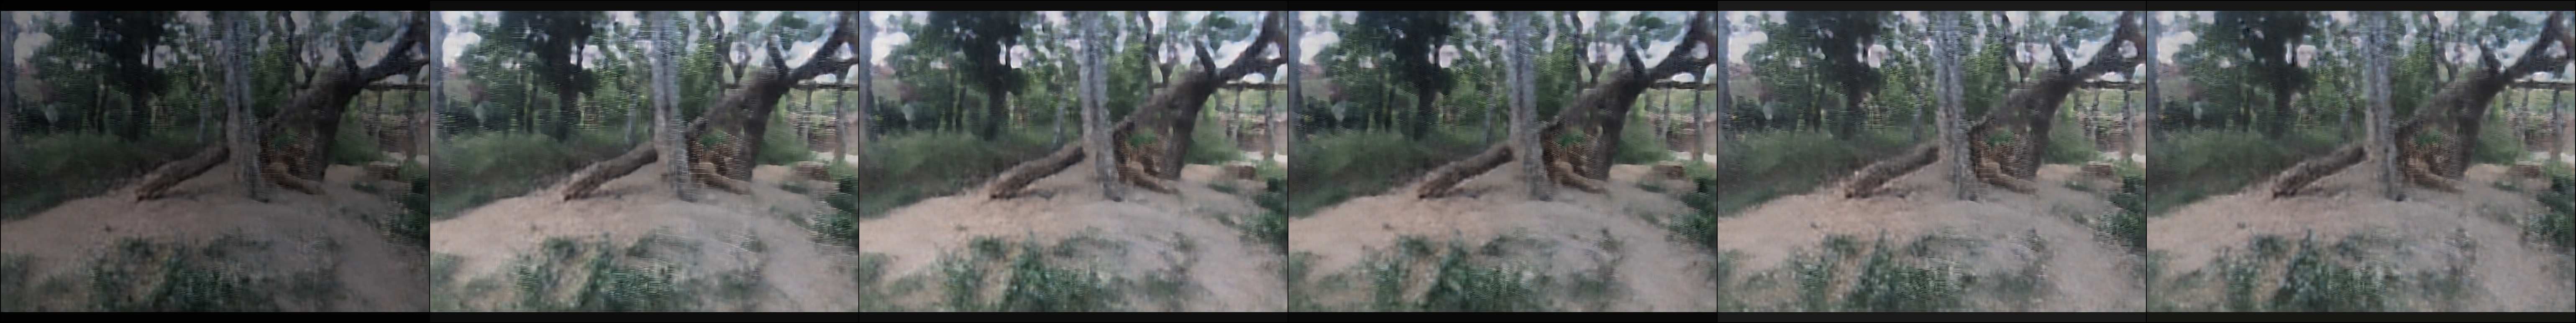
\includegraphics[width=0.75\linewidth]{figures/no_rest/prediction_432_2020-05-06 09_58_40.811600.png}
    \includegraphics[width=0.75\linewidth]{figures/reset/label_432_2020-05-04 11_19_20.713044.png}
    \end{center}
\end{frame}

\begin{frame}{Results}
    \framesubtitle{Qualitative results - with and without reset}
    \begin{center}
    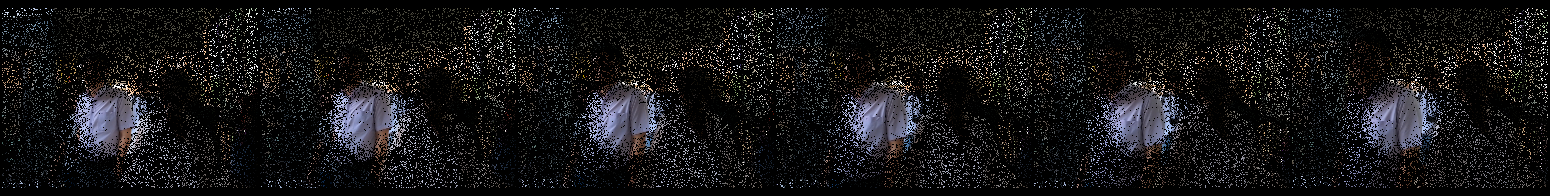
\includegraphics[width=0.75\linewidth]{figures/reset/input_83_2020-05-04 11_16_57.840082.png}
    \includegraphics[width=0.75\linewidth]{figures/reset/prediction_83_2020-05-04 11_16_53.597074.png}
    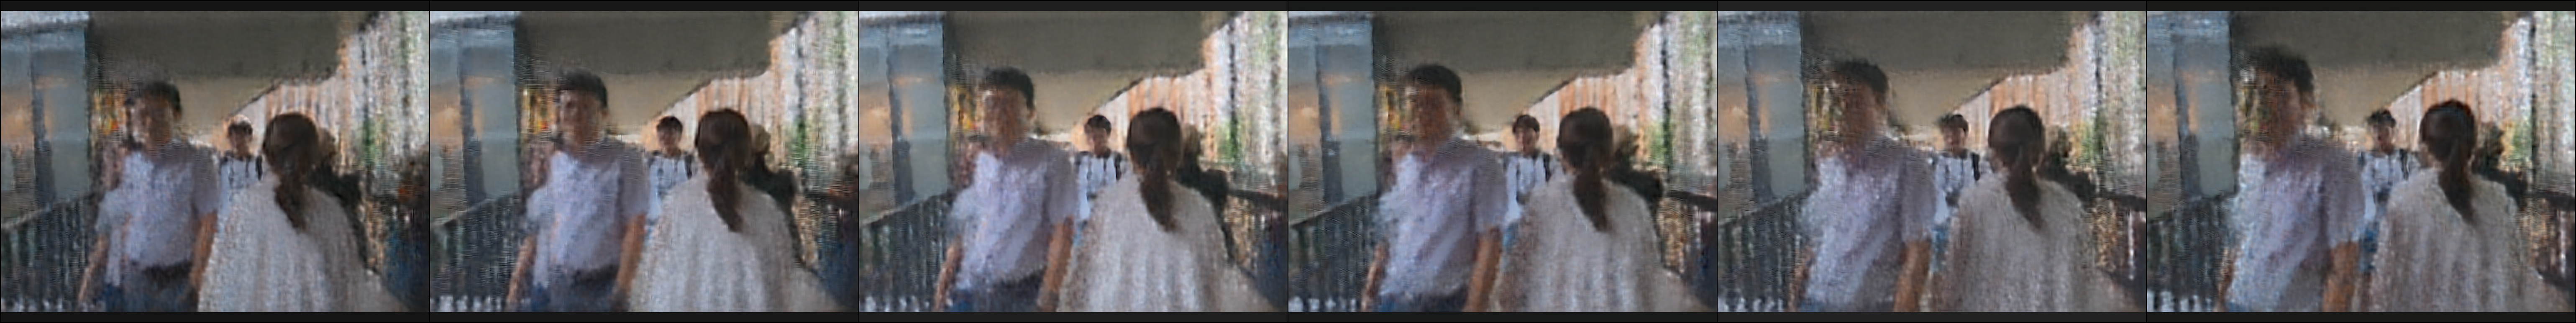
\includegraphics[width=0.75\linewidth]{figures/no_rest/prediction_83_2020-05-06 09_56_17.234900.png}
    \includegraphics[width=0.75\linewidth]{figures/reset/label_83_2020-05-04 11_16_55.895397.png}
    \end{center}
\end{frame}


\begin{frame}{Results}
    \framesubtitle{Quantitative results}
    \begin{table}[!htbp]
    \centering
    \begin{center}
        \begin{tabular}{c|c|c|c|c}
            Reset & $\operatorname{L1}\downarrow$ & $\operatorname{L2}\downarrow$ & Peak signal-to-noise ratio $\operatorname{PSNR}\uparrow$ & Structural similarity $\operatorname{SSIM}\uparrow$ \\ 
            \hline 
            \cmark & 0.0701 & 0.0117 & 22.6681 & 0.9116 \\
            \xmark & {\bf 0.061} & {\bf 0.009} & {\bf 23.8755} & {\bf 0.9290} \\ 
            \hline 
        \end{tabular} 
    \end{center}
    \end{table}
    \begin{align*}
        \operatorname{PSNR}&=10 \log_{10}\left(\frac{\max\left\{\hat{\Tensor{I}}\right\}^2}{\operatorname{L2}\left(\hat{\Tensor{I}}, \Tensor{I}\right)} \right)\\
        \operatorname{SSIM}&=\frac{4\Mean{\hat{\Tensor{I}}}\Mean{\Tensor{I}}\Cov{\hat{\Tensor{I}}, \Tensor{I}}}{\left(\Mean{\hat{\Tensor{I}}}^2 + \Mean{\Tensor{I}}^2\right)\left(\Var{\hat{\Tensor{I}}} + \Var{\Tensor{I}}\right)}.
    \end{align*}
\end{frame}

%%%%%%%%% Conclusion %%%%%%%%%

\begin{frame}{Conclusion and Possible Future Research}
    \begin{block}{Conclusion}
    \begin{itemize}
        \item Solid deep learning baseline to a novel problem
        \item Good result on the REDS dataset \cite{REDS} which can be used as a benchmark
        \item Fast inference (reconstruction network 2.3M parameters)
    \end{itemize}
    \end{block}
    \pause
    \begin{block}{Possible Future Research}
        \begin{itemize}
            \item Handle high memory consumption at training time
            \item Optimize the architecture of the reconstruction network 
        \end{itemize}
    \end{block}
\end{frame}

%%%%%%%%% References %%%%%%%%%

\section{References}

\begin{frame}[allowframebreaks]{References}
    \bibliographystyle{IEEEtranN}
    \bibliography{bib}
\end{frame}

%%%%%%%%% References %%%%%%%%%

\begin{frame}{Code Availability \& Additional Resources}
    \begin{figure}
        \centering
        \includegraphics[width=4cm]{figures/qrcode.eps}\hspace{2.5cm}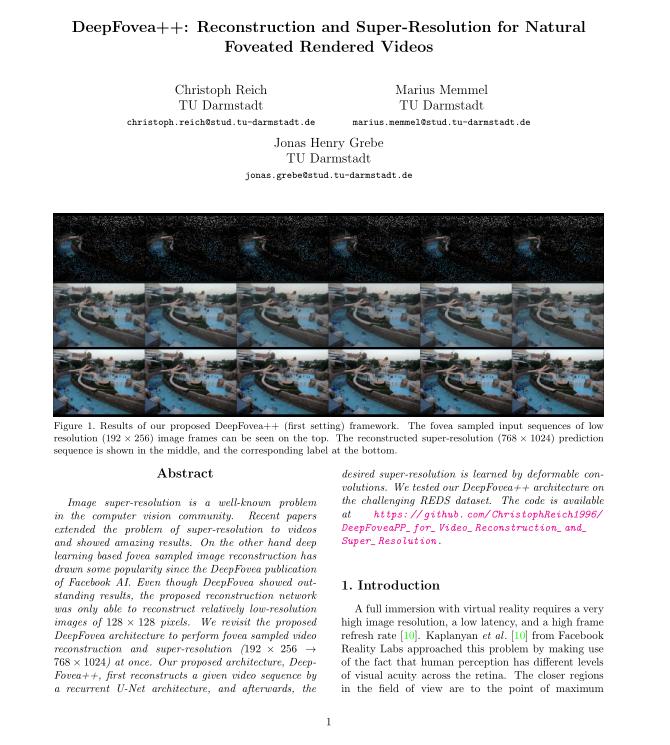
\includegraphics[width=4cm]{figures/paper.PNG}
    \end{figure}
    \begin{center}
        \begin{large}
            \url{https://github.com/ChristophReich1996/DeepFoveaPP_for_Video_Reconstruction_and_Super_Resolution}
        \end{large}
    \end{center}
\end{frame}

\end{document}
